\documentclass[12pt,a4paper,twoside]{article}

\title{Algoritmo di Kruskal}
\author{Fabio Cassini}

\usepackage[italian]{babel}
\usepackage[utf8]{inputenc}
\usepackage[T1]{fontenc}
\usepackage{graphicx}
\usepackage{amsmath,amsthm,amssymb}

\theoremstyle{definition}
\newtheorem{definition}{Definizione}[section]

\theoremstyle{definition}
\newtheorem{lemma}{Lemma}[section]

\theoremstyle{theorem}
\newtheorem{theorem}{Teorema}[section]

\begin{document}
	\maketitle
	\section{Introduzione}
	Lo scopo di questo scritto è quello di aiutare gli studenti del corso di Ricerca Operativa a meglio comprendere l'algoritmo di Kruskal visto in aula a lezione. In particolare in questa sede si presenterà l'algoritmo e si vedrà altresì il suo possibile impiego per la rappresentazione della famiglia di alberi ricoprenti di peso minimo.
	
	\section{Definizioni preliminari}
	L'algoritmo di Kruskal è un algoritmo utilizzato per calcolare gli alberi di peso minimo di un grafo non orientato e con pesi degli archi non negativi. Per descriverlo in maniera dettagliata, tuttavia, è necessario presentare alcune definizioni ed alcuni risultati preliminari.
	\begin{definition}[Grafo pesato]
		Sia $G=(V,E)$ un grafo, in cui $V$ rappresenta l'insieme dei nodi ed $E$ rappresenta l'insieme degli archi. Allora $G$ si dice \emph{pesato} se su $E$ è definita una funzione
		\begin{equation}
		\omega{} : e \in E \rightarrow \omega(e) \in \mathbb{R}
		\end{equation}
		I valori assunti da $\omega$ sono detti \emph{pesi degli archi}.
	\end{definition}
	\begin{definition}[Albero ricoprente di G]
		Sia $G=(V,E)$ un grafo non orientato e connesso. Si definisce \emph{albero ricoprente di $G$} un sottografo $T \subseteq G$ tale che
		\begin{itemize}
			\item $T$ è un albero (ovvero è aciclico)
			\item $T$ contiene tutti i vertici di $G$
		\end{itemize}
	\end{definition}
	\begin{definition}[Costo dell'albero ricoprente]
		Sia $G=(V,E)$ un grafo non orientato, connesso e pesato. Sia $T\subseteq G$ un albero ricoprente di $G$. Allora si definisce \emph{costo dell'albero ricoprente} la somma dei costi degli archi contenuti in $T$, ossia
		\begin{equation}
		\omega(T) = \sum_{e\in{}T}\omega(e)
		\end{equation}
	\end{definition}
	\begin{definition}[Taglio]
		Sia $G=(V,E)$ un grafo e sia $X\subseteq V$ un suo sottoinsieme di nodi. Si dice \emph{taglio} per $X$ il seguente insieme di archi:
		\begin{equation}
		\delta(X) = \{uv \in E : u \in X, v \notin X\}
		\end{equation}
	\end{definition}
	Presentiamo ora due risultati importanti tralasciandone la dimostrazione.
	\begin{lemma}[Lemma del ciclo]
		Sia $G=(V,E)$ un grafo non orientato, connesso e pesato. Sia $e$ un arco di peso massimo dentro ad un ciclo $C$. Allora esiste una soluzione ottima al problema dell'albero ricoprente di peso minimo che non contenga $e$.
	\end{lemma}
	\begin{lemma}[Lemma del taglio]
		Sia $G=(V,E)$ un grafo non orientato, connesso e pesato. Sia $e$ un arco di peso minimo dentro ad un taglio $\delta(X)$. Allora esiste una soluzione ottima al problema dell'albero ricoprente di peso minimo che contenga $e$.
	\end{lemma}
	Si noti come i due risultati siano uno il duale dell'altro.
		
	% Inserire definizione di arco, albero
	
	\section{Algoritmo di Kruskal}
	\subsection{Algoritmo di Kruskal in forma grezza}
	Una prima forma dell'algoritmo di Kruskal (che chiameremo informalmente \emph{in forma grezza}) viene suggerita dal costruire l'albero ricoprente di peso minimo un arco alla volta, effettuando scelte ritenute "localmente golose". Sinteticamente può essere riassunto nei seguenti passi:
	\begin{itemize}
		\item Si ordinano tutti gli archi per peso non decrescente
		\item Si aggiungono uno a uno partendo dalla soluzione vuota. In particolare:
		\begin{itemize}
			\item Se l'arco non fa ciclo lo aggiungo
			\item Se l'arco fa ciclo non lo aggiungo
		\end{itemize}
	\end{itemize}
	Alla fine dell'algoritmo si ottiene un albero perchè ci si rifiuta di inserire un arco se si vengono a creare cicli, ed è anche ottimo, visto che tutti gli archi che ci si rifiuta di inserire nella soluzione chiudono almeno un ciclo con archi presi prima di lui (che pesano dunque minore uguale di lui) e quindi esso sarà arco di peso massimo in quel ciclo; il lemma del ciclo ci garantisce pertanto che esista una soluzione ottima che non lo contenga.
	
	L'idea che sta alla base dell'algoritmo, dunque, è quella di fare un ciclo \emph{for} sulla lista degli archi e scegliere se prendere o meno un arco in base alle condizioni descritte sopra.
	\subsection{Algoritmo di Kruskal in forma completa}
	L'algoritmo descritto precedentemente è in realtà l'idea da cui partì Kruskal per sviluppare l'algoritmo che prende il suo nome. L'algoritmo vero e proprio utilizza una struttura dati di tipo \emph{Union-Find}, la quale permette di rappresentare partizioni di un insieme attraverso classi di equivalenza.
	Gli elementi fondamentali di questa struttura sono tre:
	\begin{description}
		\item[Init] permette di inizializzare l'insieme dei nodi in modo che ognuno sia rappresentante di sè stesso
		\item[Find] permette di restituire il rappresentante di una classe di equivalenza
		\item[Union] permette di unire due classi di equivalenza in una sola
	\end{description}
	A questo punto l'algoritmo si sviluppa nel seguente modo:
	\begin{itemize}
		\item Indichiamo con $A$ la soluzione ottima
		\item Per ogni vertice $v$ di $G$ $\longrightarrow Init(v)$ 
		\item Ordina tutti gli archi in ordine non decrescente di peso
		\item Per ogni arco $uv$
		\begin{itemize}
			\item Se $Find(u) \neq Find(v)$
				\subitem $A \leftarrow A \cup \{uv\}$
				\subitem $Union(u,v)$
		\end{itemize}
	\end{itemize}
	Alla terminazione dell'algoritmo si otterrà dunque un albero ricoprente di peso minimo del grafo $G$ dato in input.
	
	Per quanto riguarda la complessità computazionale dell'algoritmo di Kruskal, abbiamo il seguente risultato:
	\begin{theorem}
		Sia $G=(V,E)$ un grafo non orientato, connesso e pesato. Siano $m$ ed $n$ rispettivamente il numero di archi ed il numero di vertici del grafo. Allora la complessità dell'algoritmo di Kruskal nel caso peggiore è $O(m\log{n})$.
	\end{theorem}
	\section{Conduzione dell'algoritmo di Kruskal da parte dell'uomo}
	L'applicazione dell'algoritmo di Kruskal da parte di una persona fisica (rispetto alla sua implementazione ed esecuzione al calcolatore) genera una serie di difficoltà che sono affrontabili grazie ad un mix di esperienza, pratica ed intuito. Nella pratica, dunque, quello che si va a fare è utilizzare non l'algoritmo nella sua forma completa, ma piuttosto nella sua forma \emph{grezza} unitamente ad una serie di accorgimenti nel caso in cui ci si trovi di fronte alla possibilità di scelta tra più archi. In particolare, a questo proposito, risulta utile introdurre le seguenti due operazioni:
	\begin{itemize}
		\item Edge deletion
		\item Edge contraction
	\end{itemize}
	Con la \emph{Edge deletion} si vanno ad eliminare dal grafo tutti gli archi di peso strettamente maggiore rispetto a quelli che si vogliono studiare, mentre con la \emph{Edge contraction} si vanno a contrarre in supernodi tutti gli archi di peso strettamente minore.
	
	Sfruttando queste due operazioni congiuntamente, infatti, si riesce a "ripulire" il grafo da tutte le impurità che non interessano ai fini della scelta dell'inserimento o meno di un arco nella soluzione ottima; tuttavia si noti che se, da una parte, in questo modo si garantisce una maggior limpidezza ed eleganza concettuale, dall'altra si va a minare la sua praticità di utilizzo dall'operatore umano. Infatti, se si utilizzasse questa tecnica per ogni singola scelta di arco, il tempo di computazione aumenterebbe a dismisura. Per questo motivo ci si limita ad utilizzare questa tecnica soltanto in casi di particolare indecisione su più archi o nel momento in cui si voglia avere la certezza di aver operato correttamente.
	
	
	\section{Conduzione dell'algoritmo grezzo su un esempio}
	Vediamo l'algoritmo in funzione su un esempio passo per passo: a questo proposito si consideri il  grafo in Figura \ref{grafo}.
			
	In questo caso gli archi di peso più basso sono quelli di peso 2, e possono essere presi tutti in quanto non creano cicli. Otteniamo dunque quanto si vede nella Figura \ref{grafo2}.

	Procediamo in questo modo e, fino agli archi di peso 4, non incontriamo problemi. Arrivati agli archi di peso 5, notiamo che gli archi $EC$ e $QI$ possono essere presi in ogni caso, mentre se si decide di prendere l'arco $AC$ si è costretti a rinunciare all'arco $AB$ e viceversa (se si prende $AB$ non si può prendere $AC$ altrimenti si chiude ciclo): pertanto se ne sceglie uno dei due arbitrariamente. Analogamente si procede con gli archi $XR$, $RU$, $UY$ e $YX$ di cui è possibile sceglierne (arbitrariamente) soltanto 3 su 4. Scegliendo di prendere gli archi $AC$, $XR$, $RU$ ed $UY$ si perviene dunque alla situazione presentata in Figura \ref{grafo5}.
	
	Per quanto riguarda gli archi di peso 6, $EF$, $OM$ ed $LN$ non possono essere sicuramente presi perchè chiudono ciclo, mentre è possibile prendere soltanto uno tra gli archi $ON$, $ML$, $IH$ e $PB$ (basta prenderne due per arrivare a chiudere ciclo). Ecco un caso in cui risulta agevole l'utilizzo della tecnica deletion/contraction. In questo modo, infatti, è possibile avere un certificato di aver proceduto in maniera corretta.
	
	Per quanto riguarda gli archi di peso 7, i due archi $BQ$ non possono essere sicuramente presi perchè chiudono ciclo, mentre è possibile prendere soltanto uno tra gli archi $OW$, $WN$, $NW$, $WX$, $VR$, $ZU$ e $TY$ (basta prenderne due per arrivare a chiudere ciclo).
	
	A questo punto non è più possibile aggiungere archi senza creare cicli: dunque l'algoritmo è terminato e un albero ricoprente di peso minimo è quello presentato in Figura \ref{grafoend}.
		
	\section{Conduzione dell'algoritmo grezzo per trovare la famiglia delle soluzioni ottime}
	In questa sezione illustreremo come ad un operatore umano possa convenire l'esecuzione dell'algoritmo di Kruskal grezzo anche allo scopo di individuare la famiglia delle soluzioni ottime.
	In questo caso, risulta agevole suddividere gli archi in tre categorie:
	\begin{itemize}
		\item Archi che sono presenti in tutte le soluzioni
		\item Archi che non sono presenti in alcuna soluzione		
		\item Archi che sono presenti in alcune soluzioni ma non in tutte
	\end{itemize}
	
	Gli archi che sono presenti in tutte le soluzioni sono quelli che possono essere sempre presi in quanto non creano cicli. Una garanzia di correttezza in questo senso è data dal lemma del taglio: se si trova un taglio in cui l'arco è di peso strettamente minimo, il lemma garantisce che quell'arco sarà in tutte le soluzioni ottime.
	
	Gli archi che sono presenti solo in alcune soluzioni sono quelli più complicati da individuare, e sono quelli per cui vale la pena scomodare la tecnica del deletion/contraction.
	
	Ad esempio, consideriamo il grafo in Figura \ref{grafo}. Fino agli archi di peso 5 non abbiamo avuto alcun problema, semplicemente tutti gli archi considerati erano presenti in ogni soluzione ottima. Arrivati agli archi di peso 5, abbiamo visto come non fosse possibile prenderli tutti, ma ad esempio solo uno tra $AC$ ed $AB$ e solo tre tra $XR$, $RU$, $UY$ e $YX$: questo è facilmente dimostrabile grazie alla tecnica deletion/contraction. Infatti, eliminando tutti gli archi con peso $>$ 5 e contraendo tutti quelli di peso $<$ 5 (su cui abbiamo già lavorato) si arriva ad una situazione del tipo rappresentato in Figura \ref{contr}, in cui gli esagoni rappresentano supernodi.
	
	A questo punto è facile vedere che per la prima componente connessa è necessario prenderne solo uno su due, mentre per la seconda componente connessa è possibile prenderne tre a scelta su quattro (altrimenti in entrambi i casi si verrebbe a creare un ciclo).
	
	Analogamente si procede in questo modo ogni volta che si incontrano situazioni di indecisione: sempre continuando con l'esempio precedente, per quanto riguarda gli archi di peso 6 si ottengono due supernodi collegati da quattro archi paralleli (dunque se ne può scegliere solo uno tra i quattro) mentre per quanto riguarda gli archi di peso 7 si ottengono due supernodi collegati da sette archi paralleli (dunque se ne può scegliere solo uno tra i sette).
	
	Gli archi che non sono presenti in alcuna soluzione, infine, sono quelli che non possono essere mai presi in quanto andrebbero inevitabilmente a chiudere ciclo ed in esso sono archi di peso massimo. In questo senso, una garanzia di correttezza ci è data dal lemma del ciclo.
	
	Quanto detto fino ad adesso può essere rappresentato sinteticamente in una figura corredata da legenda, in cui ogni colore rappresenta la possibilità di scelta di quegli archi. Ad esempio per il grafo in Figura \ref{grafo}, la famiglia di archi ricoprenti di peso minimo è data dalla Figura \ref{fam} in cui:
	\begin{itemize}
		\item Gli archi in blu sono presenti in tutte le soluzioni
		\item Gli archi in nero non sono presenti in alcuna soluzione
		\item Degli archi in verde è possibile prenderne solo uno su \emph{due} per soluzione
		\item Degli archi in viola è possibile prenderne solo tre su \emph{quattro} per soluzione 
		\item Degli archi in giallo è possibile prenderne solo uno su \emph{quattro} per soluzione 
		\item Degli archi in rosso è possibile prenderne solo uno su \emph{sette} per soluzione 
	\end{itemize}
	
	Infine il numero totale di alberi ricoprenti di peso minimo è dato da $2*4*4*7=224$.
	
	\section{Figure}
	\begin{figure}[h]
		\centering
		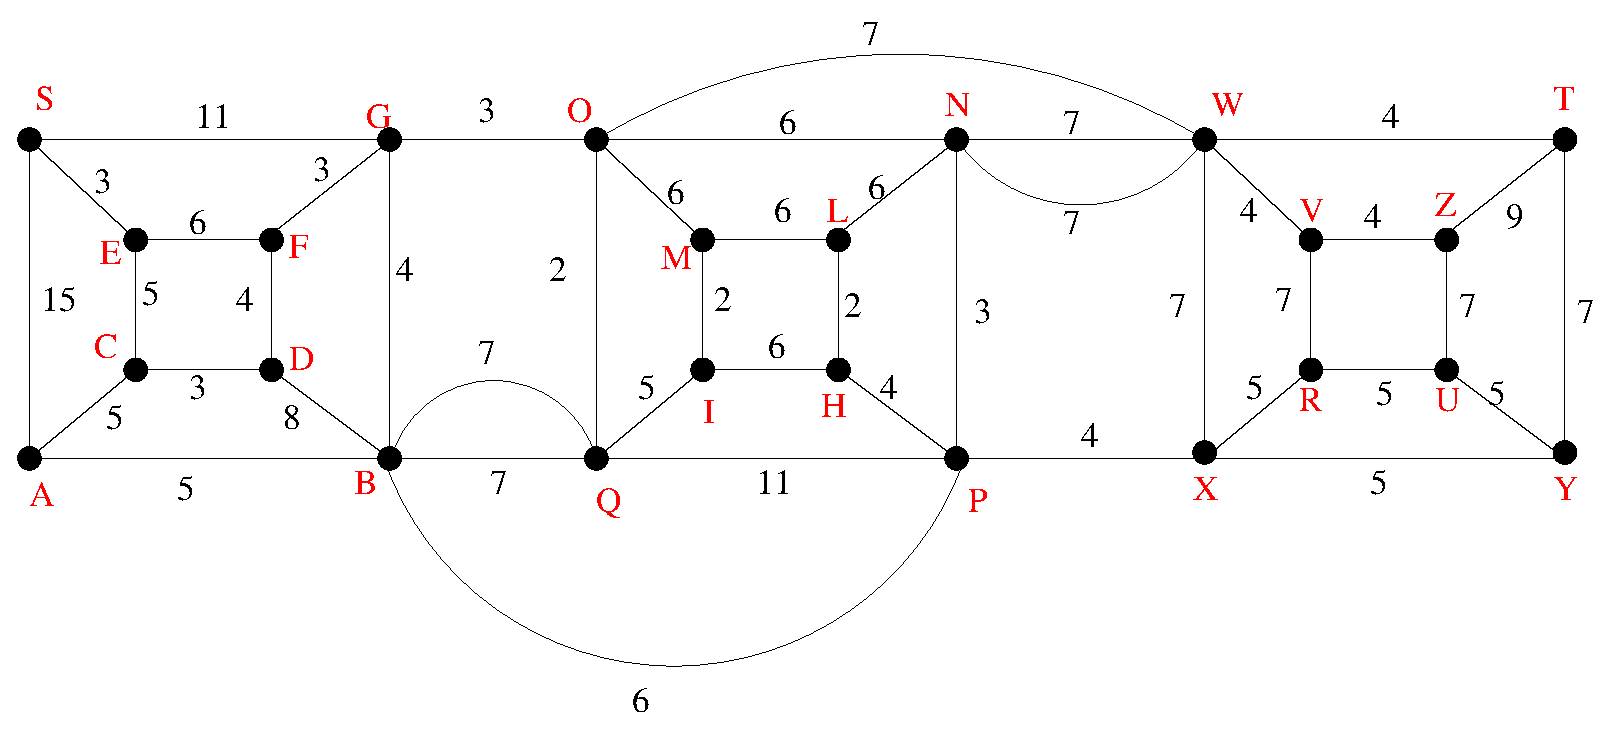
\includegraphics[width=\textwidth]{grafo_mtiff.eps}
		\caption{Grafo}\label{grafo} 
	\end{figure}	
	\begin{figure}[h]  
		\centering
		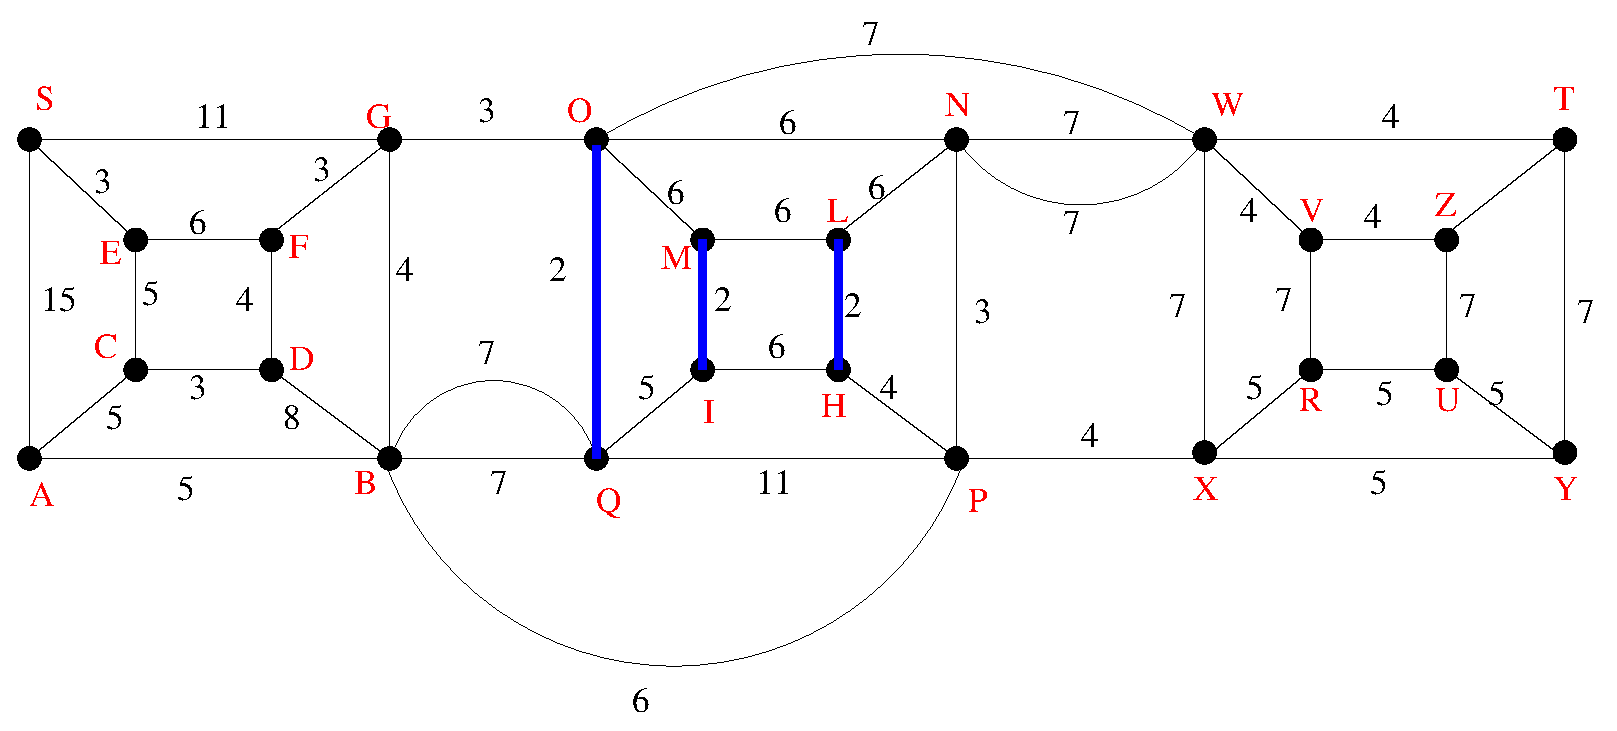
\includegraphics[width=\textwidth]{grafo2.eps}
		\caption{Costruzione dell'albero ricoprente}\label{grafo2}
	\end{figure}	
	\begin{figure}[h]
		\centering
		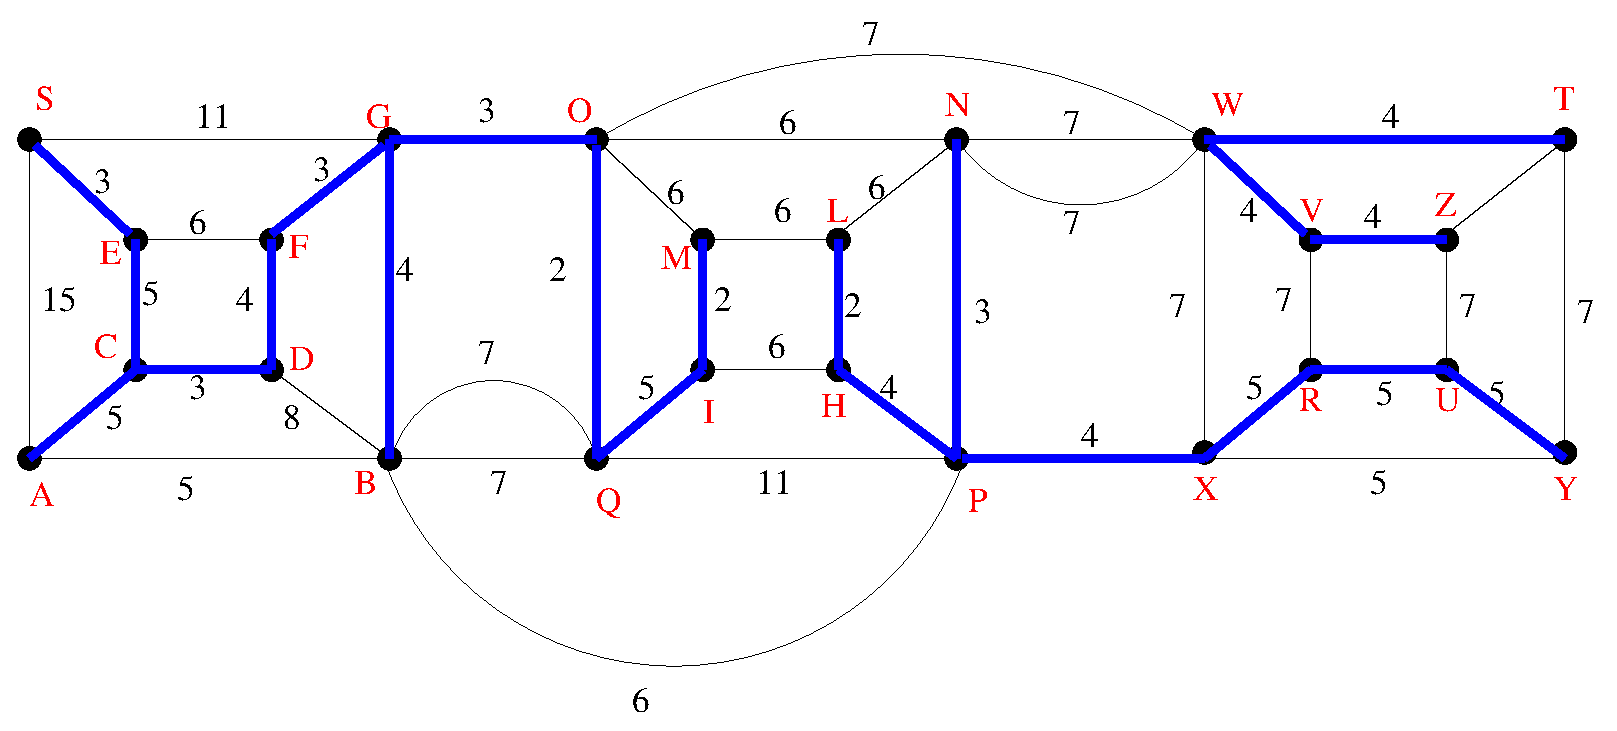
\includegraphics[width=\textwidth]{grafo5.eps}
		\caption{Costruzione dell'albero ricoprente}\label{grafo5}
	\end{figure}	
	\begin{figure}[h]
		\centering
		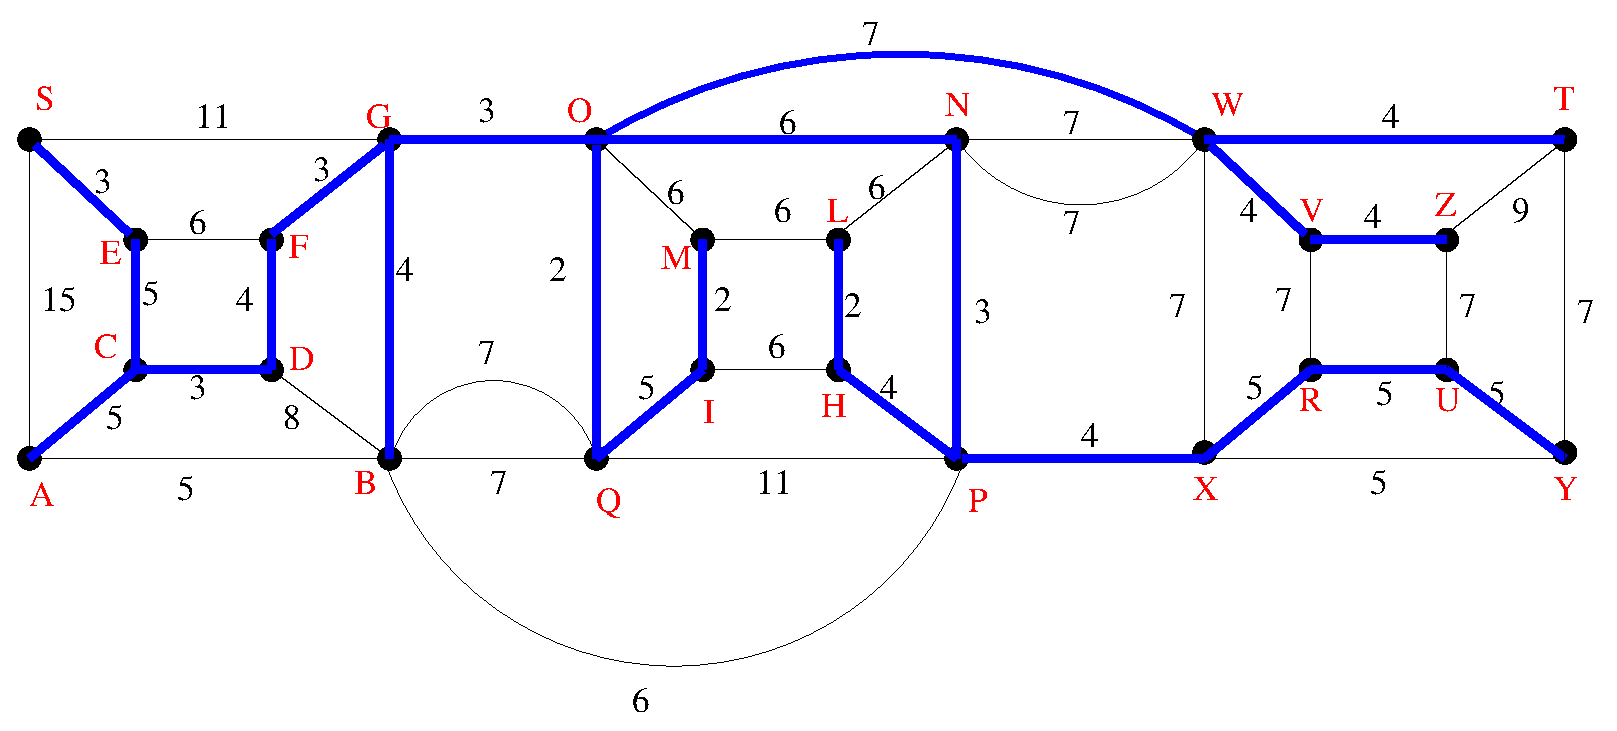
\includegraphics[width=\textwidth]{grafoend.eps}
		\caption{Albero ricoprente di peso minimo}\label{grafoend}
	\end{figure}
	\begin{figure}[h]
		\centering
		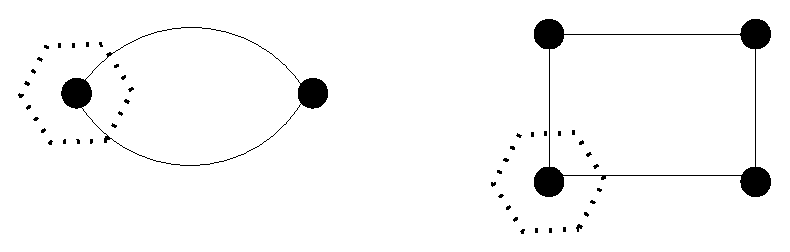
\includegraphics[width=\textwidth]{supernodi.eps}
		\caption{Edge contraction/deletion}\label{contr}
	\end{figure}
	\begin{figure}[h] 
		\centering
		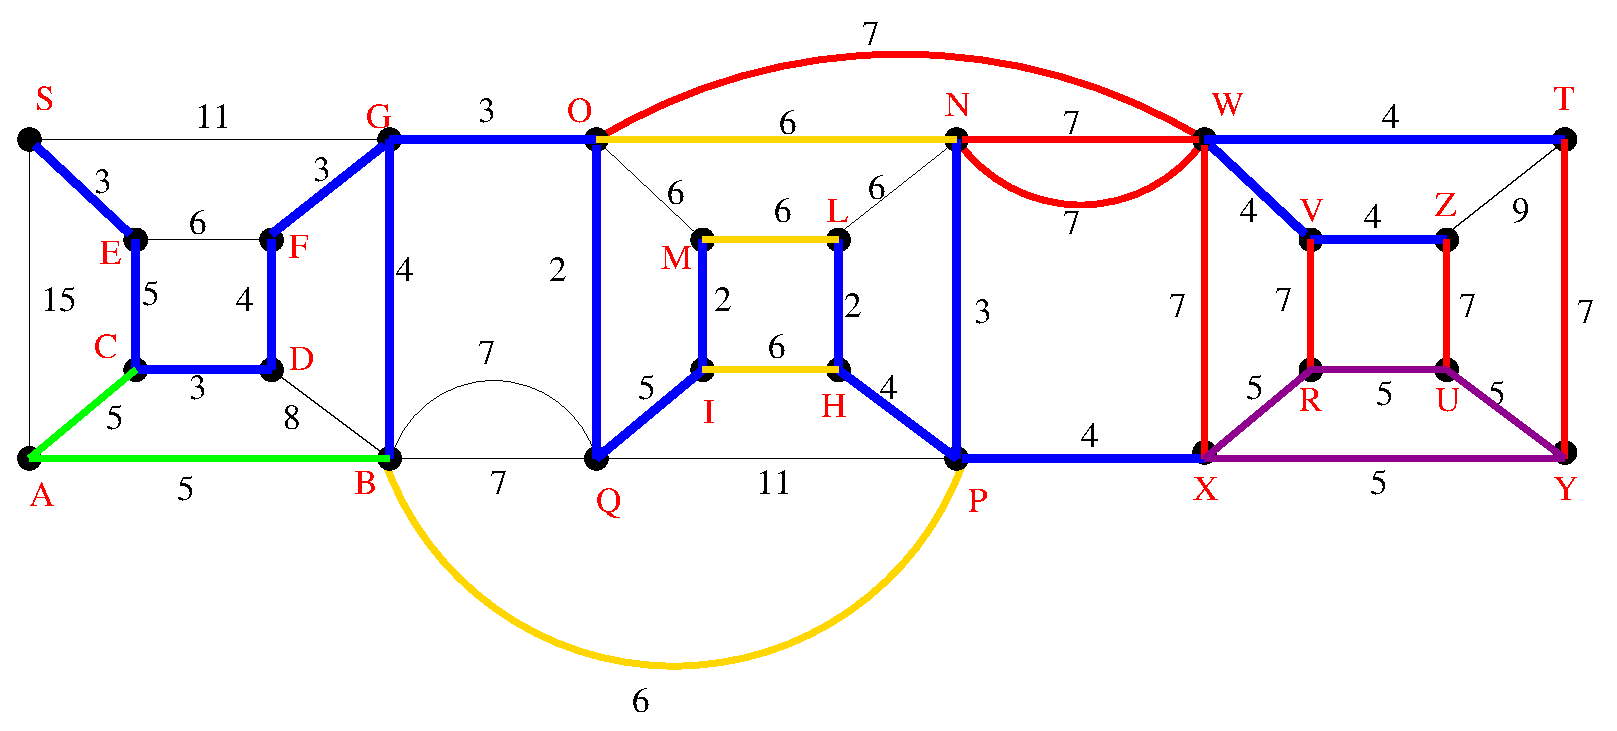
\includegraphics[width=\textwidth]{famiglia.eps}
		\caption{Famiglia di archi ricoprenti di peso minimo}\label{fam}
	\end{figure}				
\end{document}